\section{问题定义}

DiemBFT 的目标是维护具有容错能力的可编程资源数据库。该系统的核心是围绕 SMR 引擎设计的,在该引擎中,验证节点就一系列交易达成一致,并确定性地将它们按顺序应用到副本数据库中。

DiemBFT 专为经典设置而设计,其中初始系统由 n 个验证节点的网络系统组成。初始成员集在系统初始化时确定。为了模拟故障,我们定义了一个控制网络延迟和一些验证节点行为的对手。我们假设一个安全的可信主机并定义三种类型的验证节点:

\begin{itemize}
    \item 拜占庭验证节点——所有代码都由对手控制。
    \item 受损的验证节点——安全可信主机之外的所有代码都由攻击者控制。
    \item 诚实的验证节点——没有任何东西是由对手控制的
\end{itemize}

我们将诚实和被破坏的验证节点统称为非拜占庭验证节点,并假设所有验证节点都可能被破坏,但最多有 f < n/3 个拜占庭验证节点。协议属性要求诚实的验证节点永远不会提交相互矛盾的链前缀。请注意,受感染的验证节点可能会在本地提交任何内容,因为提交的信息存储在受信任的硬件模块之外。但是,受损的验证节点不会导致诚实的验证节点违反协议。


\subsection{系统模型}

\subsubsection{网络}

DiemBFT的网络模型是同步和异步模型的混合,称为部分同步。它对实际情景进行建模,其中网络经历短暂的异步阶段(例如,受到攻击)并在其余时间保持同步。

Dwork 等人介绍的部分同步设置的解决方法 [9] 将安全(在任何时候)与活跃(在同步期间)分开。DLS引入了逐轮模式,每一轮都由指定的领导者驱动。在同步期间,只要诚实的领导者出现,就可以保证进展。如果其没有出现,轮次会因超时而停止。DLS 方法是迄今为止最实用的 BFT 工作以及业内最成功的可靠性解决方案的基础,例如,谷歌 Google Chubbie lock service[3]、Yahoo’s ZooKeeper [13]、etcd [10]、Google’s Spanner[8]、Apache Cassandra[5]等。

形式上,类似于同步网络,部分同步模型假设存在传输边界$\Delta$,以及一个称为GST(全局稳定时间)的特殊事件:

\begin{itemize}
    \item GST最终会在未知的有限时间后发生。
    \item 在时间 t 发送的每条消息都必须在时间 $ max(t,GST) + \Delta$ 之前传递。
\end{itemize}

我们封装了几个与 Wire 协议相关的任务,并将其推迟到其他地方进行描述。传输(transport) 负责格式化消息并将它们序列化以通过线路传输,可靠地传递消息,以及检索传递的消息引用的任何数据,特别是块祖先。特别的,当在伪代码中处理消息时,我们假设它的格式和签名已经过验证,并且接收者已完成消息中的所引用的祖先块和其他所需数据的同步。

\subsection{技术背景}

DiemBFT基于部分同步模型中的一系列拜占庭容错(BFT)复制协议,例如[9, 6, 12, 2, 4, 14, 17, 7]。它采用了这些作品中的尖端技术,以支持可编程资源的大规模副本数据库。

\subsubsection{逐轮BFT解决方案}

实用BFT复制的经典解决方案有一个共同的基本方法。他们以循序渐进的方式运作。在每一轮中,都存在一个固定的映射,为该轮指定一个领导者(例如,通过轮次模参与者的数量,round\%n)。领导者的职责是在网络中为这个轮次填充一份唯一的提案。

如果领导者在诚实的验证节点放弃这轮投票并暂停之前,向网络发布其提案,那么领导者就是成功的。在这种情况下,诚实的验证节点会参与该回合的协议阶段。许多经典的实用BFT解决方案在每轮中分两个阶段运行,每个决策产生二次方通信成本(例如PBFT [6])。在第一阶段,法定人数的验证节点认证一个唯一的提案,形成法定人数证书或QC。在第二阶段,认证提案的法定投票数决定是否提交。未来几轮的领导者总是等待法定人数的验证节点报告他们投票选出的最高QC。如果法定人数的验证节点报告他们在第r轮中没有投票给任何QC,则这证明在第r轮中没有提交任何提案。

另一方面,HotStuff是一种三阶段BFT复制协议,在常见情况下具有线性通信开销。在HotStuff中,一轮的第一和第二阶段类似于PBFT,但第二阶段的结果是认证证书或QC的QC,而不是提交决定。在QC的QC的投票(QC的QC的QC)达到法定人数后,即可做出提交决定。

DiemBFT的灵感来自线性三阶段HotStuff,但摆脱了三阶段延迟成本。相反,当领导者还具有活性时,它保持了HotStuff的通信线性,但在视图切换协议期间允许二次通信成本,以重新获得二阶段提交的能力。

\begin{figure}[htbp]
    \centering
    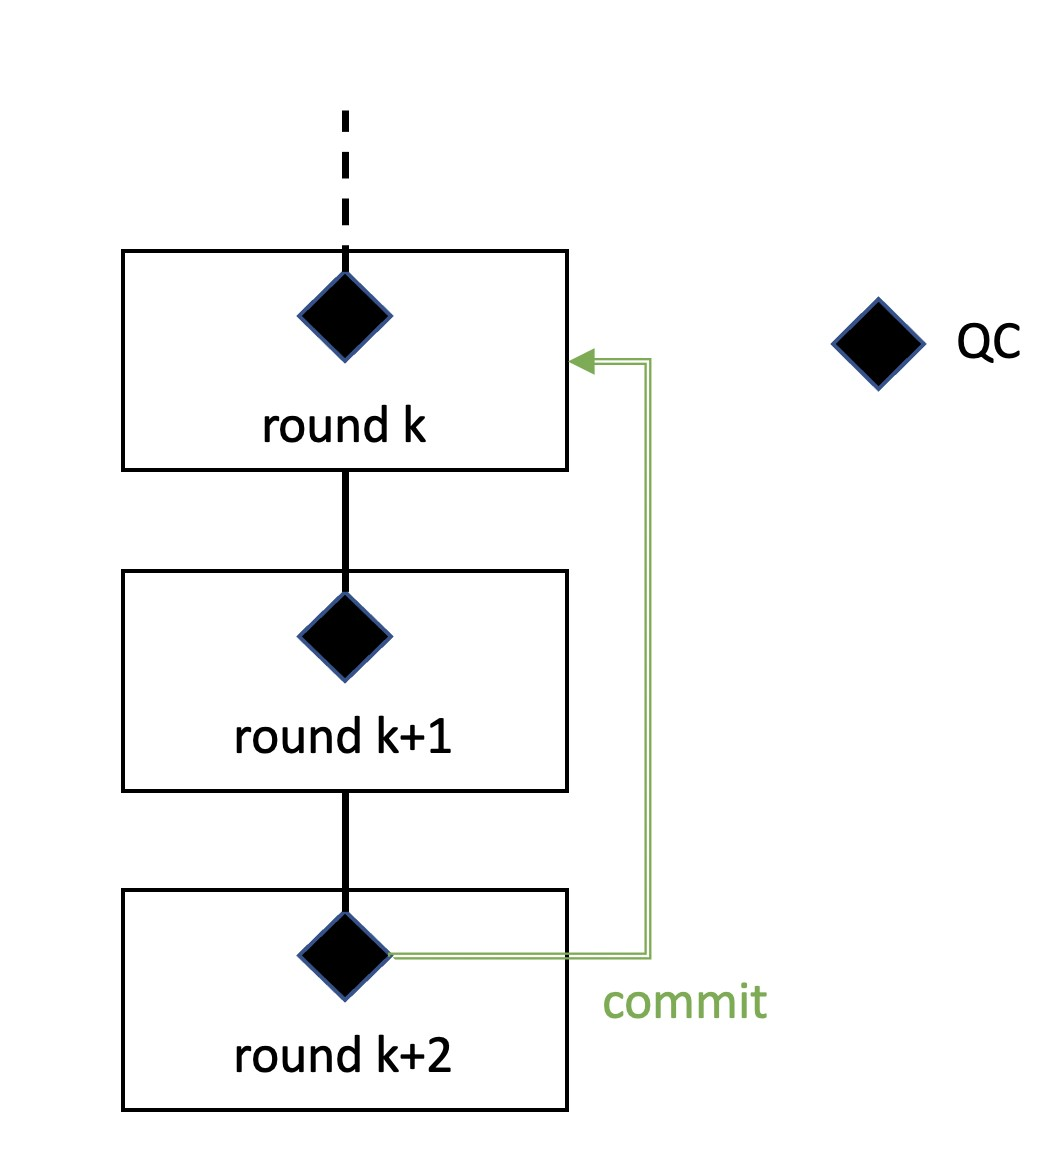
\includegraphics[width=6cm]{figures/image1.jpg}
    \caption{DiemBFT管道提案和各轮QC生成}
    \label{image1}
\end{figure}

\subsection{链}

DiemBFT 借鉴了在区块链 BFT 协议中流行的链式范式。在链式方法中,提交阶段分布在各个回合中。更具体地说,每个阶段都进行一轮并包含一个新的提案。k轮的领导者对其提案只进行了一个阶段的认证。在下一轮的k + 1中,领导者再次推动了一个阶段的认证。这个阶段有多个目的。k + 1领导者发送自己的k + 1提案。然而,它也为k提案提供了QC支持。这样,在k + 1轮认证时,会生成k + 1的QC,以及k的QC的QC。因此,在两阶段协议中,当(k + 1)提案获得QC 时,k提案可以被提交。

\subsubsection{轮次同步}

在分布式系统中,在任何时刻,验证节点都可能处于不同的状态并接收不同的消息。PBFT 通过将轮次的持续时间加倍直到观察到进展,为轮次同步提供了一种理论上的“可能性”方法。HotStuff在一个名为 PaceMaker的模块中封装了推进轮次的职责,但未说明其实现。在DiemBFT中,当验证节点放弃某一轮(比如r)时,它会广播一条超时消息,其中包含进入该轮的证书。这将使所有诚实的验证节点在传输延迟 $\Delta$ 内到达轮次r. 当从仲裁中收集超时消息时,它们会形成超时证书(TC)。TC 还包括 2f + 1 个节点在他们知道的最高轮 QC 上的签名。这也是领导者安全扩展链条的证据,即使某些验证节点锁定在比新选举的领导者更高的轮次中。为了确保GST后,所有验证节点都能够在 $\mathcal{O}(\Delta)$ 时间内为彼此形成 TC,我们使用Bracha [1]风格的机制转发超时消息。